% !TEX root = ../main.tex

% = = = = = = = = = = = = = = = = = = = = = = = = = = = = = =
% = = = = = = = = = = = = = = = = = = = = = = = = = = = = = =

\section{Introduction} 

\pw is a credit-based payment system, envisioned for small payments proposed by Rivest and Shamir~\cite{RS96}. The mechanics we will turn to later, but for now, the reader can think of tokens being issued that have some value. The key advantage of \pw is its efficiency and succinctness drawn from using only hash functions. A limitation of \pw is that tokens do not have inherent value; their value is based on the trust assumption that a counter-party will honour the value ascribed to them. With Ethereum, we can fix this issue by stapling cryptocurrency to the token through the use of a smart contract. Finally, while Ethereum already has internal functionality for payments, \ew enables payments to be made off-blockchain and settled once on-blockchain.

This transformation turns \pw from a trust-based credit system to an escrow-based payment system; not unlike offline payment channels and networks being proposed for Bitcoin (\eg the Lightning Network~\cite{PD15}). It is known that an Ethereum-based payment channel will be less complex than a Bitcoin one, since most of the complexity of Bitcoin-based payments channels comes from Bitcoin's limited scripting language~\cite{MMSH16}. \ew is a uni-directional payment channel that can be chained into a payment network and has very compact (\eg 256-bit) payments. It thus might be an interesting primitive to enhance in the same ways other payment channels~\cite{DW15,PD15} have been: adding features~\cite{KG17}, increasing efficiency~\cite{DEFM17,MBKM17}, and adding transactional privacy~\cite{GM17,MMK+17,HAB+17,RMKG18}.

\section{Background}

Beginning in the 1980s, a significant amount of the cryptographic literature has been devoted to the design of e-cash systems. In the 1990s, many startups worked toward deployment of this technology but most ultimately failed~\cite{NBFMG16}. By late 2008, when Bitcoin was first proposed~\cite{Nak08}, innovation on both the academic and commercial side of digital cash had dried up. Now Bitcoin's success has breathed new life into the field: cryptocurrencies have billion dollar market capitalizations and academic conferences like \textit{Financial Cryptography} are again publishing papers on financial cryptography. 

At first glance, Bitcoin seems like a major departure from the e-cash systems from the 80s and 90s. In reality, its `academic pedigree' is a novel combination of pre-existing ideas~\cite{NaCl17}. Similarly, researchers are re-discovering long lost ideas from the e-cash literature and finding new ways to apply them in a blockchain world. For example, blinded coins were a staple of e-cash~\cite{Cha82} that re-emerge, along with accumulators~\cite{SaTa99}, in post-Bitcoin systems like zcash~\cite{MGGR13,SCG+14}. Enabling micropayments through lottery-based probablistic payments of macropayments was explored in the 90s~\cite{Riv97,Whe97,JaOd97} and re-emerged for Bitcoin~\cite{Pash15}. In this paper, we `re-discover' the 1997 payment system \pw from Rivest and Shamir~\cite{RS96}. 

% = = = = = = = = = = = = = = = = = = = = = = = = = = = = = =
% = = = = = = = = = = = = = = = = = = = = = = = = = = = = = =

\section{Preliminaries}

\textbf{Hash chains.} A hash chain~\cite{Lam81} is constructed by iteratively applying a public one-way hash function $\Hash{}$ on a random value $s$. Let the notation $\HashN{i+1}{s} = \Hash{\HashN{i}{s}}$. A hash chain of length $n+1$ is:
\begin{equation*} \tuple{s,\Hash{s},\HashN{2}{s},\HashN{3}{s},\ldots,\HashN{n-1}{s},\HashN{n}{s}} \end{equation*}

where $s$ (technically equivalent to $\HashN{0}{s}$) is called the \textit{seed} and $\HashN{n}{s}$ is called the \textit{tip}. Given the hash is preimage resistant against a computationally bounded adversary, knowing some value in the chain $\HashN{x}{s}$ does not reveal any values `up' the chain from it, including the seed: $\tuple{s,\ldots,\HashN{x-1}{s}}$. Conversely the value $\HashN{x}{s}$ can be iteratively hashed to produce the rest of the values `down' the chain ending up producing the tip value. 

\textbf{Recognition.} If Alice meets Bob at a party, Bob can give the tip of a chain to Alice as a token~\cite{ABC+98}. Later when Bob meets Alice again, he can provide $\HashN{n-1}{s}$ as proof he is the the same person that gave her the token. On the subsequent visit, he provides $\HashN{n-2}{s}$ and so on for $n$ visits. Of course, Bob could more directly provide Alice with his public key and sign messages each visit, however hash chains avoid the relatively expensive public key operations of a signature.

\textbf{Payments.} In \pw, recognition is used for credit-based payments. A \make generates a length $n+1$ hash chain and provides a signed\footnote{The signature is only for non-repudiation, not for future authentication.} tip to a \take. They agree that each preceding value in the hash chain has a specified unit of value owed to the \take by the \make. For example, say $n$ is 100 and the value of each hash in the chain is a \$1 debt owed to the \take. To expense \$27, the \make provides $\HashN{n-27}{s}$ to the \take who will verify that hashing it 27 times produces the signed tip. The \make can increase the amount by sending further hashes, up to \$100 (the \textit{capacity}), after which, the payment channel is \textit{exhausted} and must be reinitiated.

\textbf{Payment channels.} Payment channels were reconceived for Bitcoin~\cite{DW15,PD15} to offer offline payments between Alice, Bob, and possibly with some intermediaries relaying transactions. In Bitcoin, payment channels work the same as \ew (in other words, \ew \textit{is} a payment channel) but involve setting up a number signed transactions (some pushed to the blockchain and others held in reserve) and the payments themselves are one or more full and signed Bitcoin transaction. While \ew is a payment channel, it is a simple one. It can only send payments from the \make to the \take (thus it is \textit{unidirectional}) and it can only send payments in increasing amounts (thus it is \textit{monotonic}). Making a bidirectional payment channel, where payment values can be increased and decreased arbitrarily, is interesting future work.

\label{sec:pcn}

\textbf{Pay50.} A recent blog post by Di Ferrante argues for the simplicity of Ether\-eum-based payment channels (relative to Bitcoin) and he offers a `50 lines of code' Solidity implementation of a uni-directional, monotonic channel we will name \fifty for the purposes of this paper~\cite{DF17}. As a deliberate barebones implementation, it is simple and it relies on offline payments to be signed by the sender. We describe it further in the next section. 

% = = = = = = = = = = = = = = = = = = = = = = = = = = = = = =
% = = = = = = = = = = = = = = = = = = = = = = = = = = = = = =

\section{\ew Implementation}

\ew is a line-by-line replication of \fifty, replacing the use of digital signatures with hash functions as described in the original \pw proposal. We slightly modernize \fifty to make it compliant with changes introduced in the Solidity language.\footnote{The source code of \fifty and \ew are included in the appendix.} We replicate \fifty to enable an isolated comparison between a signature-based approach (\fifty) and hash-based (\ew) approach.

The primary issue with \pw is that payments have no actual value and only represent an agreement to pay. In \ew, we staple Ethereum's internal currency ether (ETH) to the payments through a smart contract to give them real value. Thus \ew eliminates the counter-party risk in accepting payments that is inherent in \pw, and this is only possible because payments are backed by both a digital currency and a decentralized execution environment.

Both \fifty and \ew follow the standard paradigm used in the literature to eliminate counterparty risk (sometimes called \textit{claim-or-refund}~\cite{BK14}). If Bob (the \make) wants to send up to $X$ \eth to Alice (the \take), he prepays by loading $X$ \eth into a smart contract that the \take can withdraw from when specified conditions are met. The \make also sets a deadline for the \take to withdraw, after which he can release the escrowed funds back to himself. The \take checks that the contract is properly formed and funded; only then will she accept payments from the \make.

\subsection{\ew Code Design} 

\begin{Protocol*}[t!]
	 \begin{framed} \footnotesize
		\begin{compactlistn}
			\item The \make runs the constructor of \ew.
			\item The \make opens the contract by specifying the identity of \take, the validity period of the channel, how much each hash is worth, and funds the contract. The \make will send the contract address to \take. 
			\item The \take will check the parameters of the contract to ensure it is funded, how long she has to settle the account before the \make can withdraw his deposited funds, and the total amount of the deposited funds. When satisfied, she stores the hashchain tip offline.
			\item Offline, the \make will make payments by sending hash values. The \take will check that the value iteratively hashes to the tip for a correct number of iterations corresponding to amount of payment she expects. If \make wants to make successive payments, they send a new hash that represents the new total amount to be paid to the \take.
			\item At any time while the contract is open, \take can submit a hash value and receive the appropriate payment. If the \take has not run this function and the validity period expires, the \make can withdraw all the money in the contract and close it.
		\end{compactlistn}
		\normalsize \end{framed}
	\caption{The on-blockchain and off-blockchain steps in \ew payments~\label{alg:lab}}
\end{Protocol*}

As \ew is a modification of \fifty, we will discuss the design of both in parallel. Both use the constructor to initially setup the contract. In addition, they have two functions that both close the channel: one is used by the \take to claim a payment and other is used by the \make to dissolve the contract after it has timed out. \ew is summerized in Protocol~\ref{alg:lab}. The constructor for both \fifty and \ew establishes the core components of the contract:

\begin{compactlist}
\item \take: \texttt{msg.sender} for the contract creation.
\item \make: an address passed into the constructor.
\item Total available funds: the constructor allows an amount of Ether to be transferred to the payment channel contract (the constructor is marked \texttt{payable}).
\item Timeout: a validity period passed into the constructor. The contract also stores the block timestamp of when the constructor was run. These values are added together and when they exceed any future block timestamp, the self-destruct function is permitted to run allowing the \make a refund.
\end{compactlist}

Note that as implemented, the timeout functionality in both is timestamp dependent which could enable the \make to refund earlier than allowed, or alternatively be locked out from refunding, as a result of miner manipulation of the timestamps. This is feasible for adjustments of approximately 900 seconds. Therefore, the contract timeout should be considered `fuzzy' or imprecise. 

For \ew specifically (not \fifty), the constructor also establishes the payword tip and the amount of Ether each payword is worth. Consider a contract that holds 1.00 \eth in escrow and the \take supplies proof that they are entitled to, say, 0.45 of the 1.00 ETH by invoking this function. For \fifty, the proof is the claimed amount as signed by \make and the contract validates the signature. For \ew, it is a payword (\ie the output of a hash function). In this case, the \make might make a hash-chain of length 100, construct the contract with the tip, specify the value of each hash as 0.01 \eth, and funds the contract with 1.00 \eth. 

Note that the contract does not care about the length of the hash chain because there is no simple way (nor reason) for the \take to actually verify the length of the hash-chain. If it is too short, then \make cannot make payments after a certain point. If it is longer, than \take needs to stop accepting payments in excess of what she has verified to the contract to hold. Similarly, since the length of the hashchain is unknown to \take, the contract does not require a specific amount to be funded. The \take will just treat this amount as the maximum. 

%The amount of \eth held by the contract can be increased after opening, through the default function, but this requires one on-blockchain transaction and also requires the \take to reference the blockchain to see the increase. Thus, if increases are used too often, it becomes more economical to simply send \eth directly with Ethereum's built-in payment system than using \ew.

The \make can make an offline payment to the \take by sending a hash (again see Protocol~\ref{alg:lab}). Note that the hash is in no way bound to the identity of the \take---the smart contract binds the use of the hash to the \take. Next, note that technically the \take can compute the chain and submit any hash from this chain to \texttt{claim()}, however they are incentivized to send the most valuable hash. For this same reason, the \make can then later `up the payment' by sending a more valuable hash to the \take. This can be repeated until the \make runs out of hashes or \take wants to run \texttt{claim()}. This is called \textit{replace-by-incentive}~\cite{MMSH16} in the payment channel literature.

\begin{table}[t]          
\centering
%\begin{tabular}{ l | r | r | r }
%Function & Gas & ETH & USD \\ \hline
%Constructor 		&328\,637  	& 0.00433 	& \$0.908 \\
%Open 			&126\,180 		& 0.00166 	& \$0.349 \\ 
%Claim (50) 		&21\,511  	& 0.00028 	& \$0.059 \\
%Claim (100) 		&25\,772  	& 0.00034 	& \$0.071 \\ 
%\end{tabular}
\begin{tabular}{ l | r | r | r }
\ew Function & Gas & ETH & USD \\ \hline
Channel 		&318\,953 & 0.00539 	& \$0.689 \\
closeChannel (50) 		&18\,757  	& 0.00033 	& \$0.042 \\
closeChannel (100) 		&21\,907  	& 0.00038 	& \$0.049 \\ 
\end{tabular}
\setlength{\belowcaptionskip}{-5pt}
\caption{Function cost. Since closeChannel is dependent on how long the hash chain is for the claimed payment, we shows costs for length 50 and length 100.\label{table:gas}}
\end{table}

% = = = = = = = = = = = = = = = = = = = = = = = = = = = = = =
% = = = = = = = = = = = = = = = = = = = = = = = = = = = = = =

\subsection{Evaluation}

%\begin{table}[t]          
%\centering
%\begin{tabular}{ l | r | r }
%System 		& SLOC 	& Payment Size 	  \\ \hline
%\textsf{Pay50} 	& 35  	& 776 bits  		  \\
%\eww 		& 31		& 264 bits  		  \\ 
%\end{tabular}
%\caption{Comparison of code complexity and size of offline payments. Notes: (1) we modernized \textsf{Pay50} slightly; (2) both implementations comply with linter SolHint; (3) simple lines of code (SLOC) calculated by GitHub.\label{table:loc}}
%\end{table}

\textbf{Footprint.} Relative to \fifty, \ew does not add to the lines of code; in fact, it even shaves a few off. The more important property is the size of the payment sent to the receiver; this is reduced from a digital signature to a hash or from 776 bits to 264 bits. Note that it is even possible to reduce \eww to 256-bits; an extra 8 bit value representing the length of the hash from the tip is included for a more convenient loop.

\begin{figure}[t]
\centering

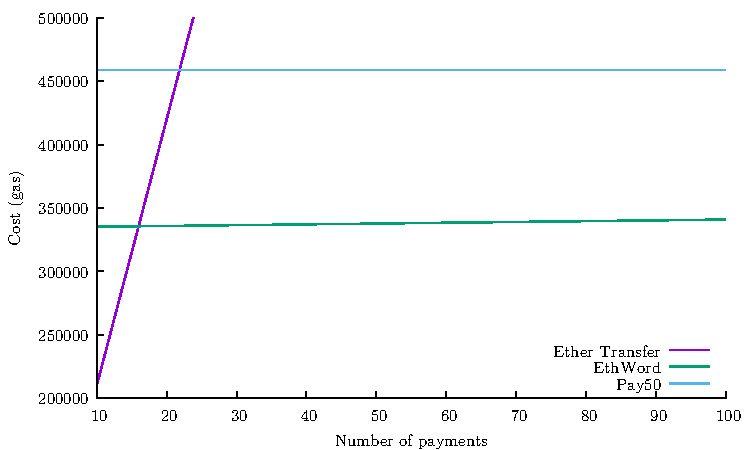
\includegraphics[width=0.75\linewidth]{figures/gas.pdf}
%\caption{The gas cost of the claim function as a function of the length of the hash chain. The gas cost of a claim in \textsf{Pay50} is around \textblue{42\,000}.\label{fig:gas}}
\setlength{\belowcaptionskip}{-10pt}
\caption{The total gas cost of running the payment channels \ew, \textsf{Pay50}, and the internal Ether Transfer as a function of the number of payments. Internal transfers are most economical up to 16 transactions, then \ew is most economical, and we extrapolate that \fifty (at a gas cost of around 460\,000) will only become more economical when the transactions exceed 1000.\label{fig:gas}}
	
\end{figure}

\textbf{Gas Costs.} As of January 15th, 2019, the weighted average price of 1 gas is $17.26\times10^{-9}$~ETH\footnote{https://ethgasstation.info/} and the exchange rate of 1 ETH to USD is \$127.85.\footnote{https://coinmarketcap.com/} Table~\ref{table:gas} shows the gas costs of each function in \ew if run successfully. The cost of the claim function includes checking if the provided payment (hash) is part of the hash chain (if when iteratively hashed, it results in the tip value). Thus the cost of claiming will vary on how many times the hash must be iterated. For example, consider a channel with 100 payment values worth 0.01 \eth each. Running claim on the payment value representing 0.05 \eth will require hashing the value 5 times. The payment value of 0.95 \eth will require 95 hashes. 

%In Figure~\ref{fig:gas}, we show the gas cost of the claim function as the number as the length of the chain varies from 1 to 100. At 100, the cost is 25\,772 which is still about half the cost of running a claim function that must verify a digital signature (\eg \textsf{Pay50} uses the \texttt{ecrecover} operation in Solidity with some additional processing logic).
Figure~\ref{fig:gas} shows the total gas cost of running the payment channels \ew, \textsf{Pay50}, and the internal  ether transfer as a function of the number of payments (from 1 to 100). At 100, the cost by \eww is 334\,236 which is still about 30\% less than the cost of running \textsf{Pay50} that must verify a digital signature (\ie \textsf{Pay50} uses Solidity's \texttt{ecrecover} with some additional processing logic).

\textbf{Contract Security.} As mentioned above, the contract depends on timestamps for allowing a refund after an elapsed time. Further, once the contract is refundable, the \take can still close the contract and receive payment assuming they have a payment proof. If \take and \make try to close the contract at the same time, transaction ordering will be arbitrary, subject to a gas auction, and subject to miner manipulation. For both of these issues, the \take simply needs to be aware. Well before the timeout, the \take has exclusive control over closing the contract. 

Last, consider a case where the \take is given a payment of 0.45 \eth from a contract holding 1.00 \eth. After receiving the 0.45 \eth at the address of the \take (call it T), note that T may be a contract address and if so, it's fallback function will be allowed to run. Logically, this function could recall close and result in an addition 0.45 \eth --- a reentrancy attack. The mitigation is the standard one: using \texttt{send} which does provide enough gas to  T's fallback function to make an additional function call. 


%In \ew, the contract is capable of paying out the \eth it holds, requiring a transfer function like \texttt{send()}. Transfer functions introduce the possibility of a reentrancy attack, particularly when the payment is intended to be less than the capacity of the channel---\eg an attack in this case might extract double, triple, etc. We implement a state machine to enforce that functions are executed in the correct order and this includes transitioning from an open state (required to enter the function) to a locked state that will encapsulate the transfer and is not a valid state for any function. This is in addition to using \texttt{send()}, which offers little gas to the contract receiving the funds. %We analyze the contract with the static analysis tool Oyente~\cite{LCOSH16} to help confirm its security against reentrancy attacks. 

%Oyente identifies a timestamp dependency since our timeout uses time (rather than block number). This would allow a malicious miner to increase or decrease the refund time by 15 minutes, which we accept. Oyente also identifies a transaction ordering dependency. \textblue{Investigate why and either fix or explain why it doesn't matter.}

%We also do other small things to ensure proper execution: (1) we whitelist addresses who can run each function, and (2) we use assertions to check invariances. For example, we provide a function to extend the validity period. A simple mistake such as using a signed \texttt{int} to represent the extension would permit a negative extension, or even using an unsigned integer without a guarantee against the integer overflow attack. These mistakes enable \make to withdraw sooner than specified --- thus we assert that extensions also increase the validity period.

% = = = = = = = = = = = = = = = = = = = = = = = = = = = = = =
% = = = = = = = = = = = = = = = = = = = = = = = = = = = = = =

\section{Discussion}

\textbf{Forming payment networks.} Consider a third party, in addition to the \make and the \take, called an intermediary. If \make establishes an \ew channel with the intermediary and the intermediary establishes an \ew channel with \take, and both channels use the same tip, then payments can be routed through the intermediary without trusting it. This requires one small modification: \take can run \texttt{closeChannel()} in both contracts. It can also admit further modifications: for example, the intermediary might modify \texttt{closeChannel()} so that it keeps some fraction of the total payout as a fee.

\textbf{Porting to Bitcoin.} Bitcoin's scripting language is purposely limited, compared to Ethereum, to ensure scripts execute efficiently and support Bitcoin's core functionality of digital money. Many \pw components are supported in Bitcoin script, including but not limited to locking transactions with a hash image that requires a pre-image to spend; and the ability to iteratively hash elements. However it does support looping nor dynamically changing how an output can be split. A moderate extension to Bitcoin's scripting language could enable \pw on Bitcoin; one proposal is MicroBTC~\cite{Wan18}.

\textbf{Micropayments.} With a total gas cost (to construct, open, and claim within a contract) of \$0.75 or more, \ew (or other Ethereum-based payment networks) are not suitable for true micropayments. Even to send \$100 of value, it represents a 0.75\% fee. The simplest internal Ethereum transaction costs 21\,000 gas so \ew will have to replace 16 transactions to pay for itself. 

\textbf{Prepaying.} A limitation that underlies almost all payment channels is the fact that payments have to be \textit{prepaid}. Without some broader economic infrastructure, payment channels are similar to using prepaid cards, something we expect compensation for (generally, customers pay for credit; preloading a card or account is giving the merchant credit which the merchant should pay for\footnote{For example, a \$50 Apple Store prepaid card might sell for \$40 or using a preloaded Starbucks app might result in rewards that can be redeemed for future purchases.}). If Alice were to pay all her bills for a single year using \ew (or other payment channel), she would have to have enough Ether for an entire year on the first day of the year. For many people, this would be a cash flow issue. 

\textbf{Trickling.} One issue in payments is fairness or fair exchange. When the payment is made on-blockchain for a token that is already on-blockchain, the swap of payment for token can be made atomic. However when the purchase is off-blockchain, either the purchased good or the payment has to be released first, leading to counter-party risk. Some purchases are divisible (\eg electricity purchased to charge an electric car) and in these cases, payment channels like \ew are useful for \textit{trickling} small payments in exchange for small divisions of the purchased good. If one party unfairly aborts, the value that is forfeited is small and bounded. Trickling can also be used for sending funds via an untrusted intermediary when the payment network approach cannot be used --- \eg if the intermediary is a mixing service that is anonymizing the payment stream amongst other indistinguishable output payment streams.

%\subsection{Re-upping}

%If Alice picks a sufficiently long hash-chain for her \ew payment channel to Bob and has on-going business with him, Alice can let Bob claim and then reconstruct a new channel. Or she might decide to continue to extend the payment channel's capacity by adding more \eth to the contract and extending it's validity. This will generally be cheaper than rerunning the constructor for a new contract (and the marginal cost of the extra iterations of the hash function, with greater payments, will have to be paid whether the channel is old or new). Thus the only reason to really close the channel is that Bob wants to recover his \eth. However if he wants to recover it to pay Carol, he can just set up a channel with Carol that forwards the payments he received from Alice. 










